\chapter{Présentation et Exploitation des Données Obtenues}
\paragraph{}
 Dans ce chapitre nous exploiterons  les données mise à notre
disposition par les autorités de l'\ac{ULPGL}. Celles-ci sont issues du
système d'information \ac{UAT}  et pour des
raisons de confidentialité nous n'avons pas eu accès à toute la base des
données nous avons juste fais une requête des données dont nous avons
besoin pour notre étude et l'administrateur a exécuté une requête vers
sa base des données et nous a fourni les données dont nous avons besoin
pour l'étude sous forme d'un fichier \ac {CSV}. Comme
souligné dans le chapitre premier ce chapitre se basera sur la
méthodologie \ac{CRISP-DM} elle sera subdivisé en différentes sections:
\begin{itemize}
	\item L'exploration 
	\item la préparation des données \cite{bookSckit-Learn}
\end{itemize}
\section{Introduction}
\paragraph{}
Les spécialités affirment que 70-80 \% du temps consacré à un projet
DataMining est alloué à la phase de l'exploration et la préparation des
données \cite{DataExpAV} , il n' ya pas des raccourcis pour cette phase et si on l'a pas
bien effectué nous risquons de nous retrouver entrain d'améliorer
l'exactitude de notre algorithme mais en vain nous serons toujours
obligées de retourner à cette phase et toutes ces techniques de
l'exploration des données pourrons nous venir en aide .\\
Les Étapes de la phase d'exploration et la préparation des donnes sont mentionnées sur la figure ci après :
\paragraph{}
En bref l'exploration des données consiste à se plonger dans le passée
pour prédire l'avenir .Souvenons nous que la qualité de notre entré
détermine la qualité de notre sortie, ces phases nous permettent
d'améliorer la qualité de notre entré en vue d'avoir une bonne sortie.
Voici les étapes de cette phase:
\begin{figure}[ht]
	\centering
	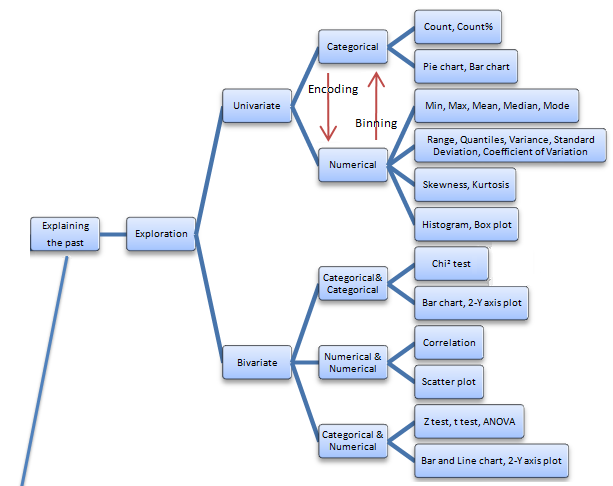
\includegraphics[width=0.5\textwidth]{fig/Exploration.png}
	\caption{Étapes de la phase d'exploration des données }
	\label{fig:imageExpSt}
\end{figure} 
\begin{itemize}
\item
  Identification des variables
\item
  Statistique Descriptive
\item
  Analyse Bi-varié
\item
  Traitement des valeur manquantes
\item
  Traitement des déviations  ou valeurs aberrantes (\emph{Outliers})  
\item
  Transformation des variables
\item
  Création des nouvelles variables
\end{itemize}
Comme nous l'avons soulignées dans le chapitre 1 ce processus est un
processus itératif et incrémentai nous exécuterons cette phase 2 a 5 fois ou plus en vue d'avoir un bon modèle.
\section{Identification des Données et des Variables}
\paragraph{}
Comme soulignées dans la phase d'introduction les données mise à notre
disposition sont sous format \ac {CSV} et nous utiliserons la librairie pandas de python pour faire l'analyse , nous utiliserons aussi d'autres libraires qui nous permettrons de faire les statistiques ainsi que les visualisations :
Nous remarquons que les données sont stocké dans un e structure de type
matricielle appelé Dataframe. \cite{pedregosa2011scikit}
Un DataFrame selon la documentation officielle de pandas est une
structure des données bidimensionnel avec des colonnes des données des différentes types . Il peut être comparée à une feuille de calcul Excel ou une table dans \ac{SQL}.
Notre ensemble d'apprentissage de départ est une matrice de 9606 lignes et  22 colonnes .\\
Chaque ligne comprend les informations d'un étudiant pour une année académique et voici la description des nos colonnes.\\ 
\begin{multicols}{2}
	\begin{enumerate}
	 \item IDENTIFICATION : contient une identification unique et anonyme d'un étudiant les noms et les matricules réels des étudiants on éé cachées
	pour des raisons de confidentialités
	
	\item BIRTHDAY : contient la date de naissance de chaque étudiant
	
	\item NAME : contient le sexe de chaque étudiant
	
	\item DIPLOMTYPE : le type de diplôme
	
	\item DIPLOMMENTION : mention de diplôme
	
	\item  DIPLOMPERCENTAGE: le pourcentage au diplôme
	
	\item DIPLOMSECTION: la section du diplôme
	
	\item DIPLOMOPTION : l'option
	
	\item  DIPLOMPLACE : l'endroit d'obtention du diplôme
	
	\item SCHOOL : l'école de provenance
	
	\item  SCHOOLPROVINCE : la province de provenance
	
	\item  SCHOOLCODE : code de l'école
	
	\item SCHOOLSTATUS : le statuts de l'école (privée , publique ,
	conventionné ,..)
	
	\item  ACADYEAR : l'année académique
	
	\item  PERC1 : pourcentage en première session
	
	\item  MENT1 : mention en première session
	
	\item  PERC2 : pourcentage en seconde session
	
	\item  MENT2 : mention en seconde session
	
	\item  FAC : la faculté de l'étudiant 
	
	\item  OPT : l'option choisie par l'étudiant
	
	\item  PROM : la promotion de l'étudiant 
	\end{enumerate}
\end{multicols}

 Comme nous pouvons le constater les colonnes 1-13 regorgent les informations que chaque étudiant donne à son inscription , ils constitueront nos variables d'entrés let es restes seront utilisées pour constituer notre variable de sortie.

Nous l'avons aussi signalé que chaque ligne comprend les information
d'un étudiant pour une année académique . Pour mener bien notre analyse nous grouperons  les informations de chaque étudiant en une ligne nos données seront groupés selon les variables d'entrées ensuite les données de sorties seront groupées selon une fonction d'agrégation prédéfinie.
Nous fairons premièrement effectuer  une analyse uni-variée  sur les données en entrées !
Soulignons que nous avons décidé de supprimer certaines colonnes n'ayant pas des informations importantes car contenant plus de 90 \% des valeurs manquantes il s'agit entre autres des colonnes suivantes :
'DIPLOMDATE','DIPLOMMENTION','DIPLOMPLACE','SCHOOLCODE'.

Après suppression les colonnes en entrée deviennent les 10 premières colonnes.

Pour une première approche nous grouperons  notre ensemble en fonction des données en entré et ensuite écrire une fonction qui va grouper les donnes de sortie la fonction de qui regroupe les données en sortie ne fait que grouper les mention , et pourcentage pour une année académique d'un étudiant dans une liste.\\ 
Après groupement en fonction des matricules nous venons de remarquer que
notre ensemble comprend 4715 lignes et 18 colonnes et c'est sera notre ensemble pour notre étude ,cet ensemble est subdivisé en variables d'entré et variables de
sortie!\\
Voici un aperçu des nos données en entrée ainsi que les données en sorties  dans  tableau \ref{tab:Dataset}
\paragraph{}
Nous venons de finir avec la présentation des nos données nous débutons avec la phase d'analyse promptement dite  des données que nous avons en entré et ensuite nous effectuerons  une analyse des données en
sortie et enfin analyse les données des sortie combinées à celles des données  en entrée.
\begin{sidewaystable}
	\centering
	\begingroup % make the next setting local
	\captionsetup{type=table} % here we want to caption a table
	\caption{Bref aperçu de notre ensemble d'apprentissage }
	\label{tab:Dataset}
	\begin{tabular}{lllllr}
		\toprule
		{} & SCHOOLSTATUS &   SCHOOL\_RIGHT &         OPTION\_RIGHT & SCHOOLPROVINCE &  DIPLOMPERCENTAGE \\
		\midrule
		45  &   protestant &         zanner &  commmerciale et adm &      NORD-KIVU &         61,000000 \\
		215 &     publique &       chemchem &            pedagogie &        MANIEMA &         51,000000 \\
		343 &   catholique &        kambali &           bio-chimie &      NORD-KIVU &         62,000000 \\
		356 &   catholique &  mwanga/ uvira &          latin philo &       SUD-KIVU &         51,000000 \\
		429 &   protestant &      maendeleo &              inconnu &      NORD-KIVU &         56,876522 \\
		474 &   protestant &      maendeleo &          latin philo &      NORD-KIVU &         56,000000 \\
		644 &     publique &          ngoma &        math-physique &      NORD-KIVU &         68,000000 \\
		645 &     publique &          ngoma &            pedagogie &      NORD-KIVU &         59,000000 \\
		\bottomrule
	\end{tabular}
	\begin{tabular}{lrlllllll}
	\toprule
	{} &   ID &                ACADYEAR &                  PERC1 &     MENT1 &                 PERC2 &       MENT2 &   FAC &      PROM \\
	\midrule
	0 &   45 &             [2013-2014] &                  [nan] &      [AA] &                 [nan] &       [nan] &  FPSE &      [L2] \\
	1 &  215 &             [2012-2013] &                  [nan] &     [ADM] &       [63.0999984741] &         [S] &    FD &      [L2] \\
	2 &  343 &             [2015-2016] &                  [nan] &      [AA] &       [52.2000007629] &         [A] &  FSEG &      [G2] \\
	3 &  356 &             [2015-2016] &                  [nan] &   [ADSTM] &       [59.9000015259] &         [S] &  FSEG &      [L2] \\
	4 &  429 &             [2013-2014] &                  [nan] &      [AA] &                 [nan] &         [A] &    FD &      [G1] \\
	5 &  474 &  [2014-2015, 2015-2016] &            [nan, 62.5] &   [AA, S] &            [nan, nan] &  [nan, nan] &    FD &  [G3, G3] \\
	6 &  644 &  [2013-2014, 2014-2015] &  [60.4000015259, 68.0] &    [S, S] &            [nan, nan] &  [nan, nan] &    FD &  [L1, L2] \\
	7 &  645 &  [2014-2015, 2015-2016] &             [nan, nan] &  [AA, AA] &  [61.4000015259, nan] &    [S, NAF] &    FD &  [L1, L2] \\
	\bottomrule
\end{tabular}
\endgroup
\end{sidewaystable}
\section{Préparation des Données}
 \subsection{Données en entré  : \emph{Inputs}}
Cette phase consistera aux traitement des valeurs manquantes et valeurs aberrantes mais aussi au nettoyage des données mal orthographiées lors de la saisie des données pour certaines attributs. 
Commençons par  Expliquer les raisons de la présence des valeur manquantes , ainsi que les données aberrantes et la manière de les traiter
\paragraph{}
Malgré la quantité croissante de données, les problématiques de données
manquantes et des valeurs extrêmes restent très répandues dans les
problèmes statistiques et nécessitent une approche particulière. Ignorer
les données manquantes et les valeurs extrêmes peut entraîner, outre une
perte de précision, de forts biais dans les modèles d'analyse et comme
signaler dans l'introduction de ce chapitre peuvent augmenter l'erreur
de prédiction.
\subsubsection{Valeurs Manquantes}
\paragraph{Cause et types des Données Manquantes} \cite{MissinVal}
Les \ac{DM} ont de multiples causes. Il peut être
impossible de contacter une personne sélectionnée pour faire partie
d'une enquête (non-réponse totale) ou un répondant peut refuser de
répondre à une ou plusieurs questions (non-réponse partielle). Une
mauvaise saisie de l'information peut également générer des \ac{DM}.
Finalement,des \ac{DM} peuvent aussi être causées par l'existence de données
aberrantes qui doivent être supprimées avant d'effectuer des analyses.
Selon les cause on classe les données manquantes selon différentes types
il existe plusieurs types de données manquantes, ils peuvent être introduit lors de :
\begin{enumerate}
\item  l'extraction des données :
il peut être possible qu'on ait des problèmes lors de l'extraction des données 
dans ce cas il es préférable de vérifier les données avec les donateurs c'est comme par exemple pour notre étude dans une première approche nous n'avons pas réussie les données des étudiants ayant passer en première session 
certaines fonctions peuvent aussi créer des données manquantes comme c'est le cas de notre fonction qui calcule les dates '
ces genres des données peuvent facilement être détecter.
\item  la collecte des données ;
c'est le cas le plus courant et il est plus facile de le détecter.
\end{enumerate}

Dans ce cas la classification la plus couramment utilisée ayant été
proposée par Little et Rubin \cite{MissinVal} : 
\begin{itemize}
	\item  \ac{MCAR} (complètement aléatoire)
	\item \ac{MAR} (aléatoire)
	\item \ac{MNAR} (non aléatoire)
\end{itemize}
\subparagraph{}
 Les DM sont MCAR lorsque la probabilité de non réponse pour une variable ne
dépend pas de celle-ci, mais uniquement de paramètres extérieurs,
indépendants de cette variable. Cela veut dire qu'il n'est pas possible
de définir un profil des individus ayant des DM et que la probabilité
des DM est uniforme. De manière générale, ce type de DM est très rare.
\subparagraph{}
Les DM sont dites MAR lorsque la probabilité de non-réponse peut
dépendre des observations mais pas des DM, par exemple s'il existe une
différence de non-réponse entre les hommes et les femmes concernant la
question du revenu, mais que parmi les hommes entre eux ou parmi les
femmes entre-elles, la probabilité d'avoir des non-réponses est
identique quel que soit le niveau du revenu.
\subparagraph{}
Finalement, les DM sont de type MNAR lorsque la probabilité de
non-réponse est liée aux valeurs prises par la variable ayant des
DM.comme par exemple pour notre cas les étudiant n'ayant pas passé tous
leurs examens à une session n'ont pas des pourcentage à cette session et
on pour mention \ac{AA} .

\paragraph{Techniques  d'imputations} 

Il existe 8 à 9 techniques  de traitement des données manquantes
largement répandues à l'heure actuelle, y compris des méthodes connues
pour être peu performantes mais cependant toujours utilisées. 
\begin{enumerate}
	\item Analyse des cas complets (CC)
	\item Imputation par la moyenne (MEAN) : c'est la
	méthode que nous utiliserons par défaut
	\item Imputation par la médiane
	(MED)
	\item  Imputation par régression simple (REG)
	\item Imputation multiple par Markov Chain Monte-Carlo (MCMC)
	\item  Imputation par le plus proche
	voisin (KNN)
	\item Imputation multiple par un algorithme basé sur le
	bootstrap, approchant des résultats de l'algorithme EM (EM)
	\item Imputation multiple par ``Predictive Mean Matching'' (PMM)
\end{enumerate}
Toutes ces techniques existe sont implémentées dans les librairies que nous
utilisons.\\
Dans ce travail selon le cas nous fairons  une imputation par la
moyenne ou par analyse des cas complets mais soulignons qu'il faut bien
réfléchir avant d'utiliser une imputation par la moyenne car il a une
mauvaise influence sur la variance
\subsubsection{Valeurs aberrantes ou extrêmes ou outliers}
Une valeur aberrante est une valeur qui diffère de façon significative
de la tendance globale des autres observations quand on observe un
ensemble de données ayant des caractéristiques communes. Par exemple
dans l'analyse des pourcentage du diplôme à l'EXETAT nous avons trouvé
des diplôme qui ne sont pas dans l'intervalle 0 à 50 \% des étudiant
avec des diplômes de 634\% ou des diplômes de 0\%

Voici quelques remarques à considérer pour les valeurs aberrantes :
\begin{enumerate}
	\item Les valeurs aberrantes ne sont pas forcément erronées. Dans certains
	cas, la valeur aberrante doit être acceptée comme une indication
	intéressante. par exemple après analyse on trouve une étudiant âge de 60
	ans! 
	\item Il ne faut pas adopter une attitude radicale de rejet, ou
	d'inclusion systématique des valeurs aberrantes. Le rejet systématique
	peut entraîner la perte d'informations réelles Le rejet des valeurs
	aberrantes a des conséquences statistiques non négligeables car
	l'analyse est ensuite faite sur un échantillon censuré qui n'est plus
	aléatoire.
\end{enumerate}
En fonction des circonstances, il existe des méthodes,
dites robustes, qui prennent en compte toutes les données mais
minimisent l'influence des valeurs aberrantes. 
L'apparition de valeurs aberrantes est due à diverses sources de natures différentes, d'où la
complexité de l'examen des valeurs aberrantes.

Pour détecter les valeurs manquantes nous avons utiliser les techniques
suivantes :

\begin{enumerate}
	\def\labelenumi{\alph{enumi})}
	\item
	Contrôle sur le domaine des valeurs : Exemple : Pour la variable «
	DIPLOMPERCENTAGE », une borne maximale (100 \% ) est connue et la
	valeur minimale est de 50 . Les valeurs supérieures à 100 et
	inférieur à 50 sont considérés comme aberrantes.
	\item
	Détection graphique : Pour détecter la présence de valeurs aberrantes
	On a utilisé :
\end{enumerate}

\begin{itemize}
	\item
	Boxplot
	\item
	diagramme de dispersion des observations classées en fonction de leur
	rang
\end{itemize}

\paragraph{Traitement des valeurs aberrantes :}
\begin{enumerate}
	\item  Les valeurs aberrantes pouvant provenir d'erreurs de saisie, on le traite séparément
	en étudiant cas par cas.C'est cette technique que nous utiliserons 
	pour certaines valeurs du pourcentage de diplôme.
	\item On les rejette et on applique ensuite une des méthodes d’imputation (moyenne,médiane…) vues pour les valeurs manquantes.
	\item  On adopte des méthodes qui diminuent leur impact au cours des analyses statistiques :la médiane
\end{enumerate}
Voici Un aperçu des nos colonnes avec données manquantes et données aberrantes
au tableau \ref{tab:MisisnV} .
\begin{table}
\centering
\begingroup % make the next setting local
\captionsetup{type=table} % here we want to caption a table
\caption{Statistiques Des Données avec Valeurs manquantes et abberantes}
\label{tab:MisisnV}
\begin{tabular}{lrlllllll}
	\toprule
	{}& IDENTIFICATION   &  BIRTHDAY &  DIPLOMPERCENTAGE \\
	\midrule  
count  &   4038.000000 & 4038.000000      & 4038.000000\\
mean   &   8792.137692  &   26.072022       &  57.749876 \\
std   &    2333.542658   &  3.957584     &    95.088746\\
min   &     215.000000    &20.000000     &     0.000000\\
25perc  &     7310.250000 &   24.000000     &    52.000000\\
50perc   &   9181.500000  & 25.000000      &   55.000000\\
75perc  &   10540.750000   & 27.000000     &    60.000000 \\
max  &    12360.000000  &  58.000000      & 6053.000000\\
\bottomrule
\end{tabular}
\endgroup
\end{table}

Ce tableau décrit toutes les informations possibles sur les données
continues et de prime à bord nous sommes à mesure de constater certaines
incohérences sur les pourcentages du  diplôme qui ont un maximum de 6053 et un
minimum de 0 qui est vraiment impossible car le diplôme en RDC dois être
compris entre 50 et 100 \% !Nous visualiserons ces incohérence de
plus prêt avec des box-plots.

\begin{figure}[ht]
	\centering
	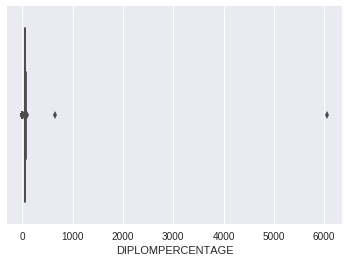
\includegraphics[width=0.5\textwidth]{fig/AGEPlot1.png}
	\caption{Box Plot Attribue Diplôme Pourcentage  }
	\label{fig:AgeBXPlot1}
\end{figure} 

\begin{figure}[ht]
	\centering
	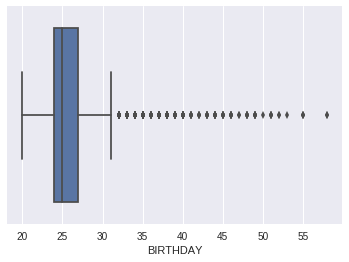
\includegraphics[width=0.5\textwidth]{fig/PercetagePlot.png}
	\caption{Box Plot Attribue  Age  }
	\label{fig:PercBXPlot1}
\end{figure} 
Au vu de ces courbes nous remarquons que l'attributs diplôme pourcentage
dispose de beaucoup des déviations. Nous avons pu corriger au cas par cas en remplaçant les valeurs aberrantes par leurs valeurs exactes et d'autres par la moyenne comme il n'était pas nombreux
\subsubsection{Données mal orthographiées }
Dans notre première analyse nous avons remarqué que certaines  attributs ont des valeurs très désorganisées et vraiment dispersé et ce
qui a une mauvaise influence sur le calcul de l'entropie et ainsi sur
les algorithmes du Machine Learning . Nous pouvons aisément constater
que ce problèmes est du à des fautes d'orthographes commise lors de la
phase de saisie des données et ainsi pour continues nous devons essayer
de corriger ces erreurs et bien organisé les données . 

Par exemple pour la variable diplôme section on a pu voir les valeurs suivantes : 'TECSC', 'Techniqe',
'TECHN IQUE',technique','TCH' qui sont saisie pour la même et unique
section 'techniques' mais avec différentes erreurs d'orthographe. \\
Pour l'attribut SCHOOL nous avons obtenus les valeurs suivantes :
'matanoia', 'metanoia', 'metonoina', '\%etanoia', 'meta' pour la seule école 'metanoia'
Nous avons aussi remarqué ces genres d'incohérence pour les autres attributs catégorielles.  
Après analyse , nous avons pu détecter qu'il étaient  dus à des erreurs d'orthographe.
Ces genres d'erreur de notation ont pour conséquence le fait qu'il font
augmenter l'entropie de nos colonnes et ainsi pénalisent nos algorithmes
surtout lorsqu'on travaille avec les arbres de décisions .Nous avons
procédé à un nettoyage automatique qui a consisté en un groupement des
valeurs proches en utilisant la distance de Leveinstein :\cite{LevStack}combinée au  clustering par l'algorithme d'affinity propagation,et
ainsi qu'un nettoyage manuel pour arranger les données à la fin de
cette phase nous avons obtenus des données moyennement propres et bien
nettoyées avec une entropie faible.
 \subsection{Données en sortie: \emph{Outputs}}

 Dans cette partie , nous préparerons notre ensemble de sortie en
 construisant nos variables de sortie , celles-ci seront constituées à
 l'aide des divers fonction qui nous aideront à déterminer pour une année
 si sur base des résultats que nous avons si un étudiant est passé en
 première session, s'il a distingué ou bien s'il a échoué, nous
 déterminerons enfin le pourcentage obtenu.
 
 Notons que nous nous sommes butés à 2 grands problèmes concernant les
 données obtenus et qui risquent de biaiser nos calculs,  ils constituent en fait les limites de ce travail . 
 \begin{enumerate}
 	\item Nous n'avons
 	pas pu obtenir le pourcentage final de certains étudiants ayant échoué
 	ou abandonné leurs études avant la fin de l'année académique , ces
 	étudiants qui après la seconde session sont AA (Assimilé aux Ajournées )
 	n'ont pas de pourcentage final pour palier à ce problème , nous avons
 	remplacer cette valeur manquante par une valeur aléatoire choisie entre
 	45\% et 53\%   ce qui représente l'échec!
 	\item  Pour nous étudiant le
 	nombre des années académiques pour lequel nous avons le résultat n'est
 	pas le même pour certains étudiants nous avons des informations pour une 
 	année académique, d'autres pour 2 , etc. Pour palier à ce problème nous
 	avons utilisé des ratios pour nous valeur de sortie qui consister à
 	diviser le nombre sur le nombre des année académiques que l'étudiant a
 	passée à la faculté.
 \end{enumerate}:
  Voici sur la figure \ref{tab:Output1} à  quoi ressemble notre ensemble d'apprentissage pour chaque année académique :
\begin{table}
	\centering
	\begingroup % make the next setting local
	\captionsetup{type=table} % here we want to caption a table
	\caption{Sortie Pour Chaque Année Académique}
	\label{tab:Output1}
	\begin{tabular}{lrlrlrllllllr}
		\toprule
		{} &   ID &   YEAR &      PERC1 &  MENT1 &      PERC2 & MENT2 &   FAC & PROM &  Echec & Pass1erSession & Distinction &  PercFinal \\
		\midrule
		0 &   45 &  2013-2014 &        NaN &     AA &        NaN &   NaN &  FPSE &   L2 &   True &          False &       False &  43,000000 \\
		1 &  215 &  2012-2013 &        NaN &    ADM &  63,099998 &     S &    FD &   L2 &  False &          False &       False &  63,099998 \\
		2 &  343 &  2015-2016 &        NaN &     AA &  52,200001 &     A &  FSEG &   G2 &   True &          False &       False &  52,200001 \\
		3 &  356 &  2015-2016 &        NaN &  ADSTM &  59,900002 &     S &  FSEG &   L2 &  False &          False &       False &  59,900002 \\
		4 &  398 &  2012-2013 &  65,099998 &      S &        NaN &   NaN &  FSDC &   L2 &  False &           True &       False &  65,099998 \\
		5 &  429 &  2013-2014 &        NaN &     AA &        NaN &     A &    FD &   G1 &   True &          False &       False &  41,000000 \\
		6 &  474 &  2014-2015 &        NaN &     AA &        NaN &   NaN &    FD &   G3 &   True &          False &       False &  46,000000 \\
		7 &  474 &  2015-2016 &  62,500000 &      S &        NaN &   NaN &    FD &   G3 &  False &           True &       False &  62,500000 \\
		\bottomrule
	\end{tabular}
	\endgroup
\end{table}
 Nous avons ensuite constituer notre ensemble d'apprentissage finale en groupant ces données pour chaque année académique et en évaluant 
 la moyenne des pourcentages obtenus à la fin de chaque année académique  et nous l'appellerons \textbf{\ac{CGPA} }par analogie avec le système anglophone, \emph{elle constituera notre variable de sortie principale}  nous l'accompagnerons de 3 autres variables entre autre :
 \begin{itemize}
 	\item
 	DistinctionRatio : Le nombre de fois que l'étudiant a distingué
 	divisé par le nombre des années académique
 	\item
 	EchecRatio : Le nombre de fois que l'étudiant a échoué divisé par le
 	nombre des années académique
 	\item
 	PassAstSessionRatio : Le nombre de fois que l'étudiant est passée en
 	première session divisé par le nombre des années académique
 \end{itemize}
\begin{table}
	\centering
	\begingroup % make the next setting local
	\captionsetup{type=table} % here we want to caption a table
	\caption{Sortie Chaque étudiant avec des Ratio}
	\label{tab:Output2}
	\begin{tabular}{lrrrrrr}
		\toprule
		{} &   ID &       CGPA &  DistinctionRatio &  EchecRatio &  NADYEAR &  Pass1stSessionRatio \\
		\midrule
		0 &   45 &  43,000000 &                0, &         1,0 &         1, &                  0,0 \\
		1 &  215 &  63,099998 &                0, &         0,0 &         1, &                  0,0 \\
		2 &  343 &  52,200001 &                0, &         1,0 &         1, &                  0,0 \\
		3 &  356 &  59,900002 &                0, &         0,0 &         1, &                  0,0 \\
		4 &  398 &  65,099998 &                0, &         0,0 &         1, &                  1,0 \\
		5 &  429 &  41,000000 &                0, &         1,0 &         1, &                  0,0 \\
		6 &  474 &  54,250000 &                0, &         0,5 &         2, &                  0,5 \\
		7 &  526 &  65,000000 &                0, &         0,0 &         1, &                  1,0 \\
		\bottomrule
	\end{tabular}
	\endgroup
\end{table}
Nos 3 derniers ratio sont des nombres variant qui peuvent prendre ses
différents valeurs :
\begin{itemize}
	\item 0 :signifie que l'étudiant a un ration de 0 
	\item  1 :signifie ration: 1/1,2/2,3/3,4/4
	\item  0.25 : 1/4
	\item  0.3333: 1/3
	\item  0.5:2/4 ou 1/2
	\item 0.66666 :2/3
	\item 0.75:3/4
\end{itemize}
 Nous allons appréhender ce problème en
terme de classification donc nous allons affecter des lettre à ces
ratio: 
\begin{itemize}
	\item 0: G
	\item  1:A
	\item  0.25 : F
	\item  0.333:E
	\item  0.5:D 
	\item 0.666:C
	\item 0.75:B
\end{itemize}
qui
correspondent aux classes respectifs!
Pour conclure cette analyse des données de sortie nous pouvons conclure que notre travail sera d'une part une tache de régression mais aussi d'une classification à multiples classes.
 \section{Analyse des données}\label{analyse-des-donnuxe9es}
\paragraph{}
Cette phase comprend une analyse statistique bi-varié et uni-varié nous
visualiserons les résultat à l'aide des graphiques . Dans cette partie
nous utiliserons beaucoup plus la statistique descriptives et la statistique inférentielle
Comme nous  pouvons le remarquer notre ensemble d'apprentissage
comprend à la fois des données numériques (continues ) ainsi que des
données discrètes catégories. voici comment nous procéderons 
\subsection{Analyse Uni-Varié}
Dans cette partie nous effectuerons les statistiques descriptives pour chaque variable .
\begin{enumerate}
	\item
	\emph{\textbf{Variable Numériques ou continues : }}Pour les données continues nous
	essayerons de comprendre la tendance et la dispersion des nos
	variables .les métriques utilisées sont sur la figure suivante: 
	\begin{figure}[ht]
		\centering
		\includegraphics[width=0.5\textwidth]{fig/DataExploration.png}
		\caption{Techniques d'exploration des données en entré }
		\label{fig:DataExplora}
	\end{figure}
	En bref nous examinerons le moyenne , le mode , l'écart-type et la
	variance , nous conterons aussi les variables nous effectuerons  les
	visualisations avec des box-plot! cette étape nous sera aussi utile
	dans le traitement des valeur manquantes et des valeurs aberrantes!
	\item
	\emph{\textbf{Variable catégorielle ou quantitative :}} Pour les données discrètes nous
	 utiliserons  les tables des fréquences pour comprendre la distribution de
	chaque catégorie nous pour aussi voir le pourcentage de chaque
	catégorie , les histogrammes et bar char seront utilisées.
\end{enumerate}
Commençons par l'analyse des attributs numériques age et pourcentage à l' \ac{EXETAT} 
\paragraph{L'AGE et Le Diplôme Pourcentage}
Voici un bref aperçu des statistiques descriptives de ses variables  à la figure\ref{tab:DescribeData}
\begin{table}
	\centering
	\begingroup % make the next setting local
	\captionsetup{type=table} % here we want to caption a table
	\caption{Statistiques Des Données }
	\label{tab:DescribeData}
	\begin{tabular}{lrr}
		\toprule
		{} &  DIPLOMPERCENTAGE &          AGE \\
		\midrule
		count &       4715,000000 &  4715,000000 \\
		mean  &         56,878914 &    24,732768 \\
		std   &          5,756663 &     4,621602 \\
		min   &         50,000000 &    18,000000 \\
		25\%   &         52,000000 &    22,000000 \\
		50\%   &         56,000000 &    24,000000 \\
		75\%   &         60,000000 &    27,000000 \\
		max   &         86,000000 &    59,000000 \\
		\bottomrule
	\end{tabular}
\endgroup
\end{table}
\subparagraph{AGE}

Nous avons calculer l'age en se basant sur la date de naissance et la date d'aujourd'hui.signalons que cet attributs disposait des valeurs manquantes au début et on était imputer par la moyenne , comme nous pouvons le voir à la figure\ref{tab:DescribeData}  nos étudiant disposent en moyenne d'un age de 24 ans avec une variance de 4,5 le moins âgé a 18 ans et le plus âgé a 59 ans.
On peut aisément que l'age suit une distribution normale . 
\begin{figure}[!htbp]
	\centering
	\subfloat[Box-Plo det  l'age ]{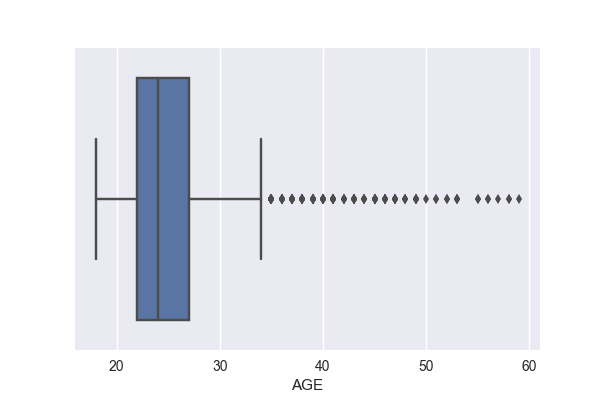
\includegraphics[width=0.4\textwidth]{fig/AGE.png}\label{fig:Agea}}
	\hfill
	\subfloat[distribution de l'age ]{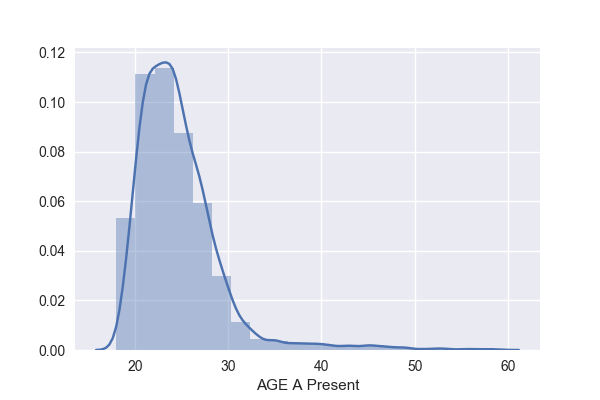
\includegraphics[width=0.4\textwidth]{fig/AGEDist.png}\label{fig:Ageb}}
	\hfill
	\caption{Graphiques de l'attributs age}
\end{figure}
\subparagraph{Pourcentage du diplôme}
Après nettoyage et contrairement à la figure\ref{tab:MisisnV} on a constater qu'après nettoyage la moyenne est de 56,8 \% avec unn écart type de 5,7 le minimum de 50 \% et un maximum de 86\% .
les graphiques représentent les informations sur l'age  son à la figure\ref{fig:Pourcentagea} et la figure\ref{fig:Pourcentagea}
\begin{figure}[!htbp]
	\centering
	\subfloat[Box-Plot du Pourcentage du diplome ]{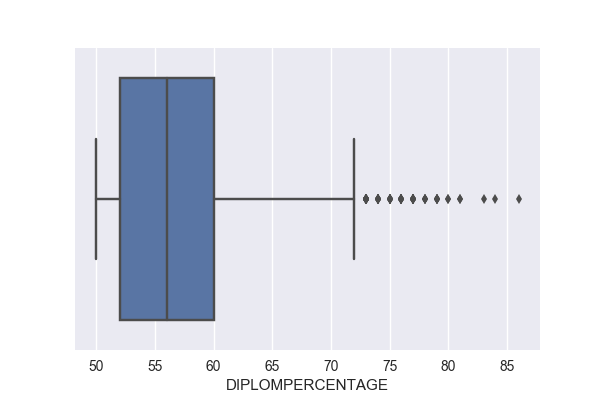
\includegraphics[width=0.4\textwidth]{fig/dipomePourcentage.png}\label{fig:Pourcentagea}}
	\hfill
	\subfloat[distribution du Pourcentage ]{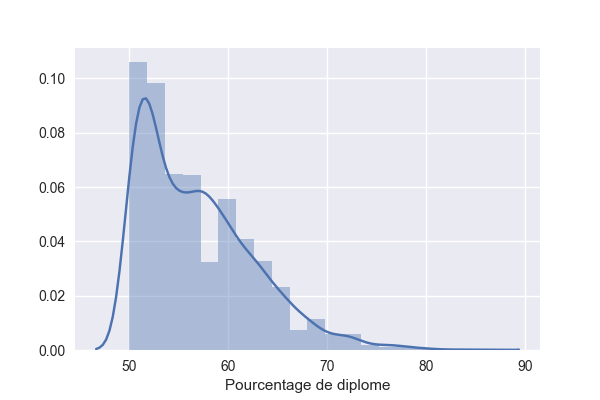
\includegraphics[width=0.4\textwidth]{fig/diplomePercentageDis.png}\label{fig:Pourcenategb}}
	\hfill
	\caption{Graphiques de l'attributs du Pourcentage à l'examen d'état }
\end{figure}
\subparagraph{Le Sexe des étudiants}
	\begin{figure}[!htbp]
	\centering
	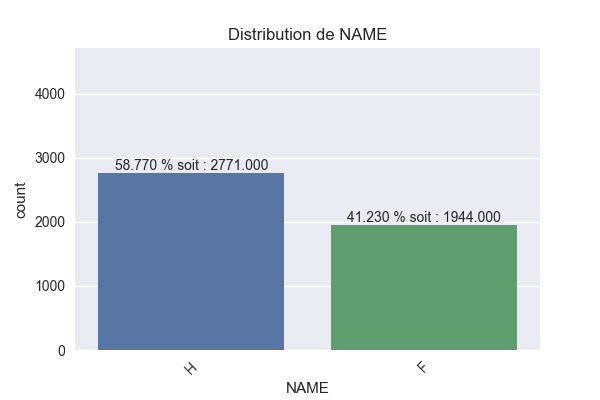
\includegraphics[width=0.5\textwidth]{fig/NAME.png}
	\caption{Distribution du sexe des étudiants }
	\label{fig:SEXE}
\end{figure}
La  figure\ref{fig:SEXE} nous donne la  répartition de sexes dans notre ensemble d'apprentissage on peut aisément constater qu'il n'est pas si déséquilibre que ça!, le
genre est vraiment respecté avec 41\% dés nouveaux étudiant étant de
sexe féminin.
\subparagraph{le type d'école}
\begin{figure}[!htbp]
	\centering
	\makebox[\textwidth]{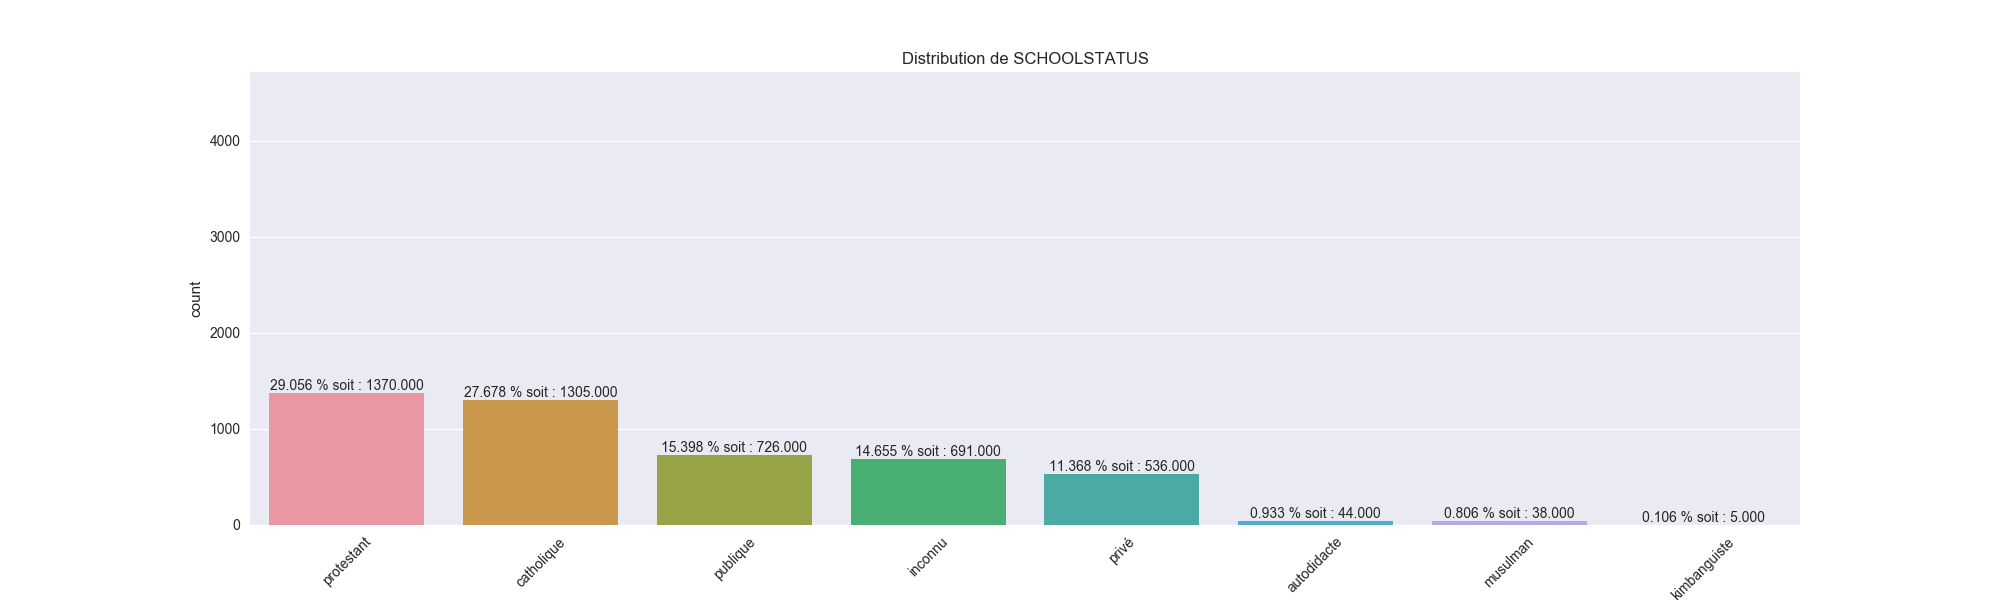
\includegraphics[width=\paperwidth]{fig/SCHOOLSTATUS.png}}
	\caption{Différente statut de l'école de provenance }
	\label{fig:SchoolStatus}
\end{figure}
 Dans la figure\ref{fig:SchoolStatus} nous pouvons remarquer aisément que 29\% des étudiants
proviennent des écoles dites protestantes , 27\% viennent des écoles
catholiques , 11\% des écoles privé , 15 des écoles publiques mais aussi
il ya des étudiants venant des autodidactes , ceux provenant des écoles
musulmanes et kibanguistes mais en proportion vraiment négligeable.
\subparagraph{l'Option de provenance}
Nos étudiants proviennent des 33 options différentes:

\begin{figure}[!htbp]
	\centering
	\makebox[\textwidth]{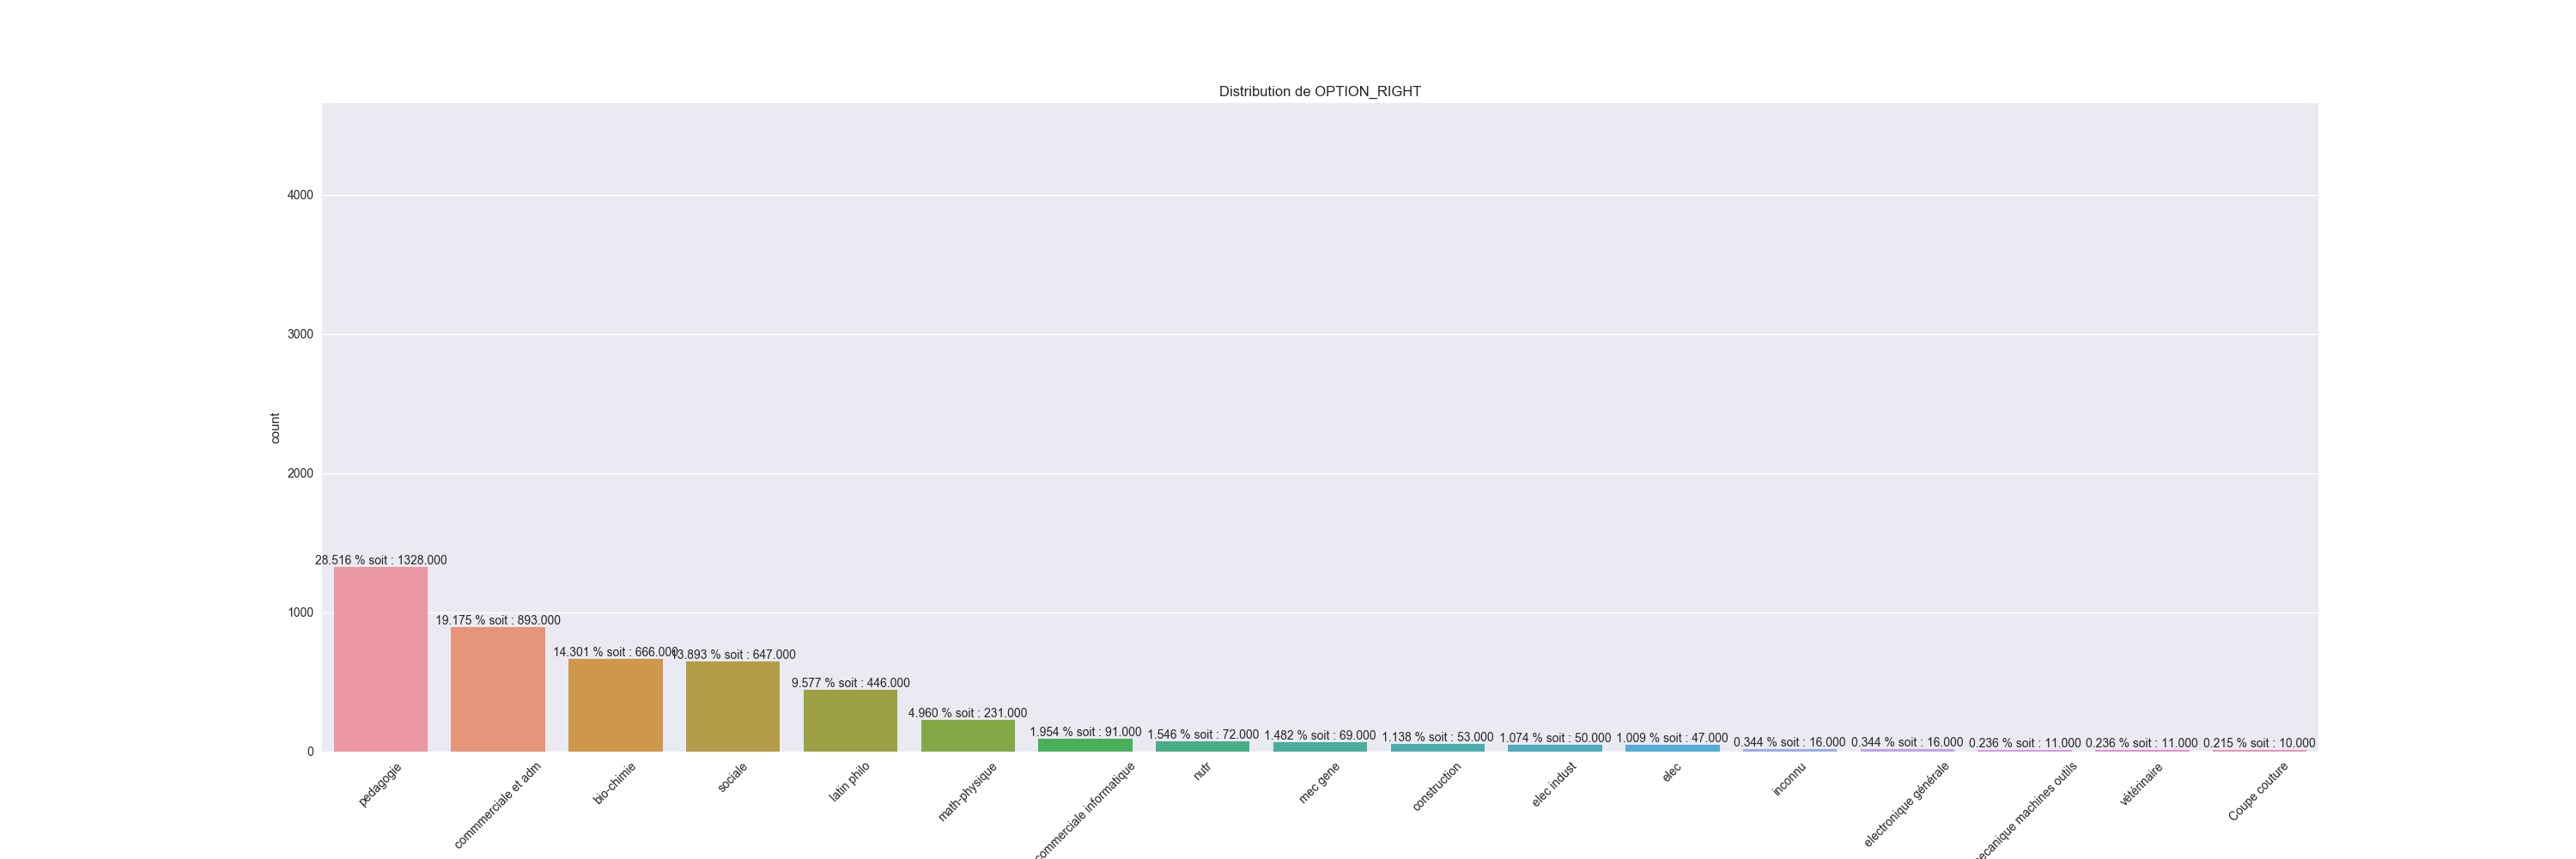
\includegraphics[width=\paperwidth]{fig/OPTION_RIGHT.png}}
	\caption{l'option suivie à l'école secondaire }
	\label{fig:Option_right}
\end{figure}
Sur la figure \ref{fig:Option_right} nous pouvons remarquer que la majeure partie des
étudiants de notre étude proviennent de la section pédagogique avec
environ 28\% ensuite vienne la section commerciale et administrative
avec 19\% , ensuite  sociale avec 13\%, scientifique bio-chimie avec 14
\% ensuite viennent les  autres différentes options avec des valeurs
inférieurs à 5\%.
\subparagraph{Attribut School}\label{attribut-school}
cette attributs comprend les valeurs de l'école de provenance des nos
finaliste combiné avec l'attributs SCHOOLSTATUS  il joue un rôle
important dans notre étude.
nous pouvons aisément remarquer que les élèves proviennent de 594 écoles
différentes sur la figure \ref{fig:SCHOOL} nous visualiserons les écoles
les plus représentées.
\begin{figure}[!htbp]
	\centering
	\makebox[\textwidth]{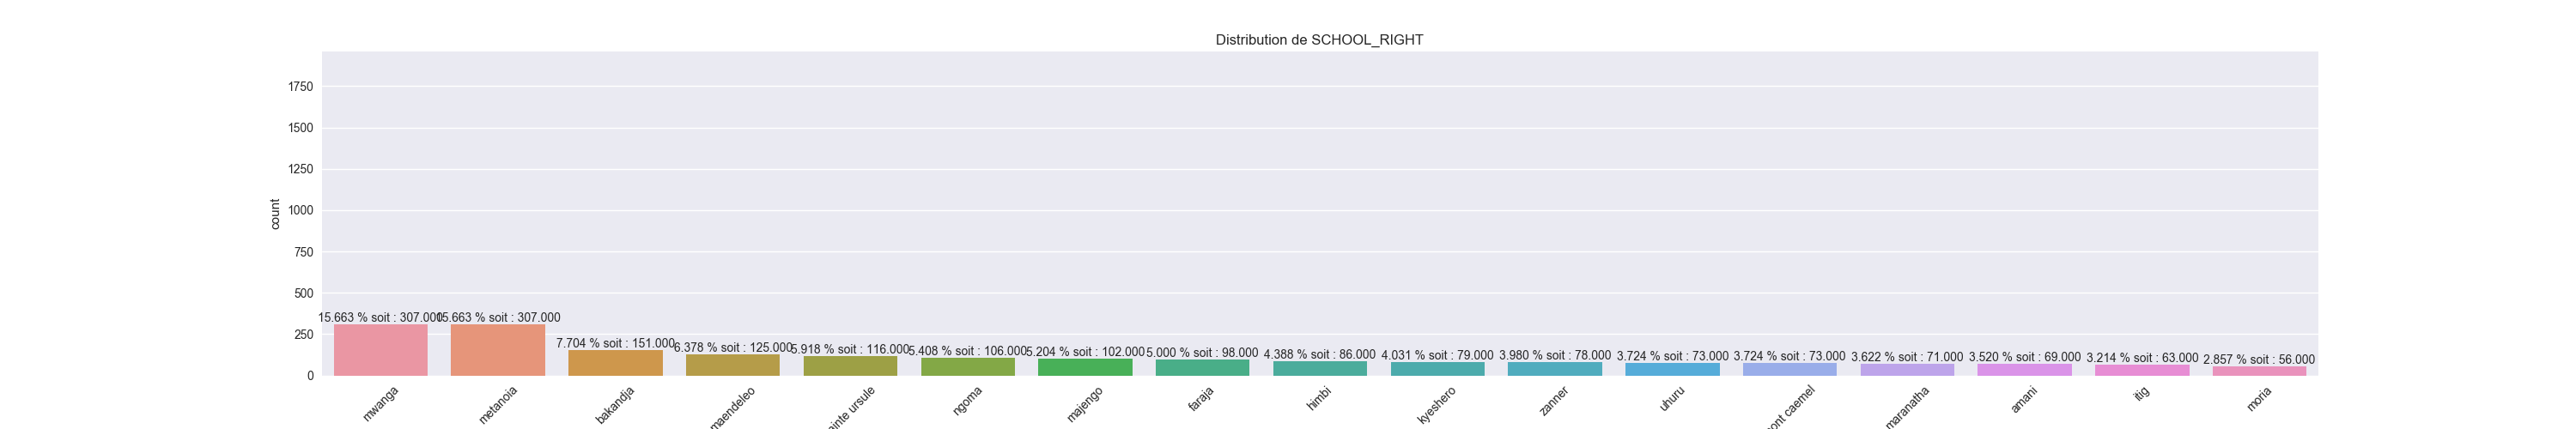
\includegraphics[width=\paperwidth]{fig/SCHOOL_RIGHT.png}}
	\caption{les écoles de provenances  }
	\label{fig:SCHOOL}
\end{figure}
Nous pouvons remarquer aisément que le top 10 des écoles de provenance
est constituer de grandes écoles de la ville de Goma avec l'institut
metanoia et le collège mwanga en tête de liste avec l'institut mwanga et
metanoia en tête de liste avec 15\% chacun ensuite vienne l'institut
bakanja avec 6\% ensuite vienne maendelo, le lycée sainte ursule et
l'institut de Goma avec 6\%, 5\% et 5 \% respectivement et d'autres
école se partagent le reste de 50\%.
\subparagraph{Attribue SCHOOL Province}
\begin{figure}[!htbp]
	\centering
	\makebox[\textwidth]{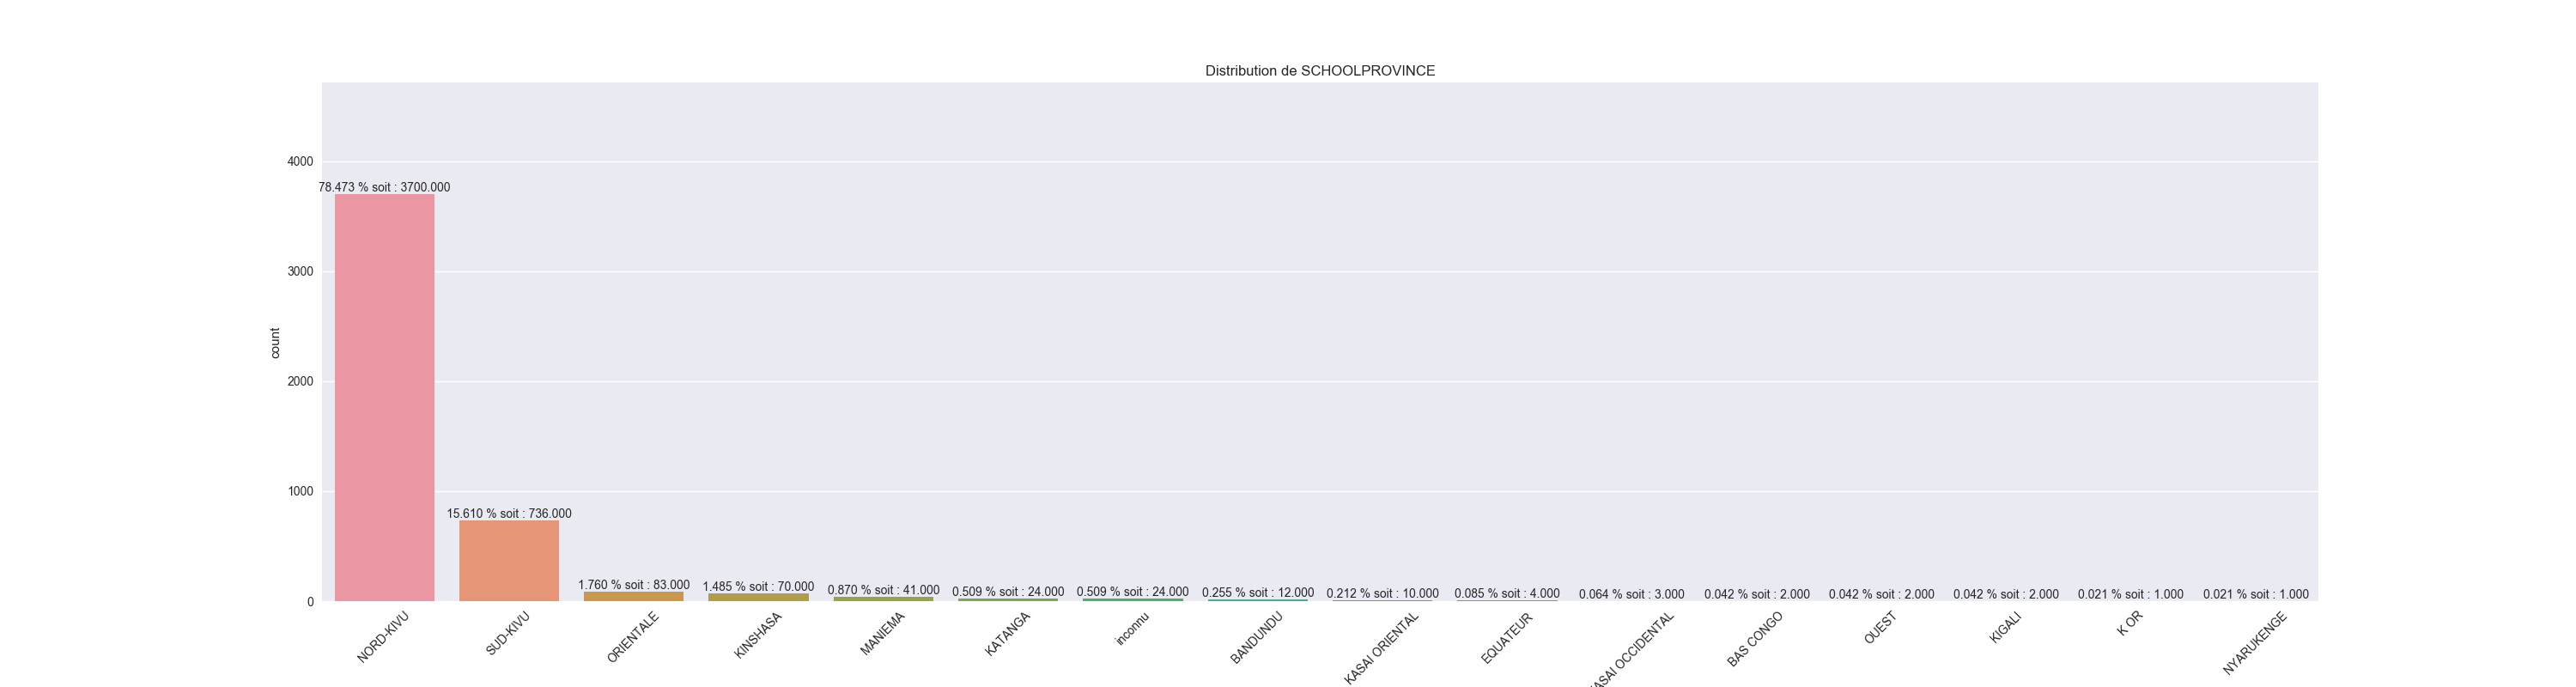
\includegraphics[width=\paperwidth]{fig/SCHOOLPROVINCE.png}}
	\caption{les provinces de provenances des étudiants   }
	\label{fig:SCHOOLProvince}
\end{figure}
A la figure \ref{fig:SCHOOLProvince} nous pouvons aisément constater que 75 \% des étudiants
de l'\ac{ULPGL} proviennent de la province du nord kivu mais il ya une autre
catégorie provenant  du Sud Kivu soit 15\% le reste des étudiants  provient des autres provinces de la \ac{RDC}.
\subparagraph{Attribue Faculté}
Pour finaliser l'analyse uni-variée de nos données en entrée nous jetterons un coup d'œil sur la colonne Fac qui contient la faculté choisie par l'étudiant.
Voici comment elle se présente a la figure \ref{fig:FAC}:
\begin{figure}[!htbp]
	\centering
	\makebox[\textwidth]{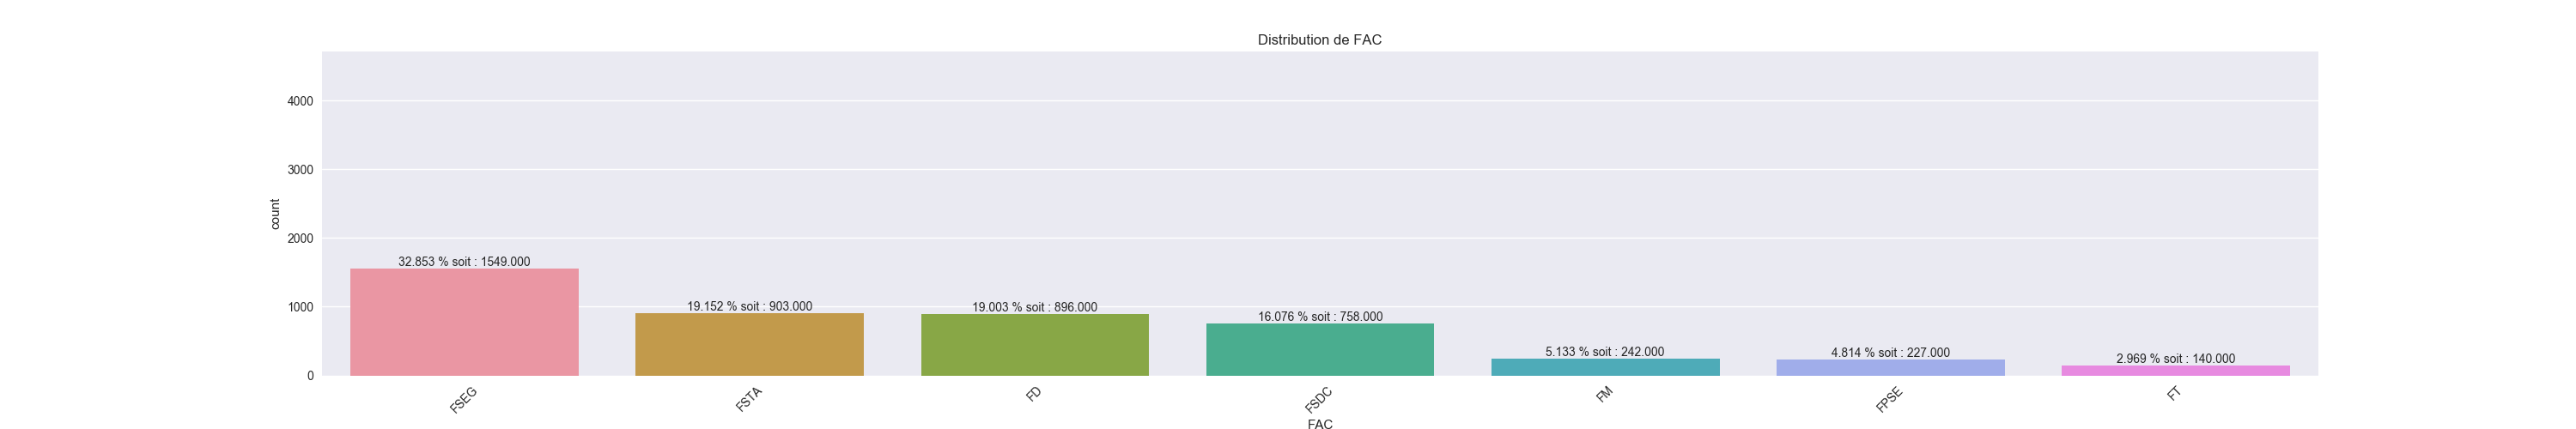
\includegraphics[width=\paperwidth]{fig/FAC.png}}
	\caption{les Facultés }
	\label{fig:FAC}
\end{figure}
 Nous remarquons la distribution des valeurs pour
l'attributs faculté des étudiants: - FSGEG: 32,8\% , FSTA : 19,153\% , FD
:19\% -,FSDC :16\% ,FM : 5\% ,FPSE : 4\% ,FT :3\%
\subsection{Analyse Bi-variée}
C'est une technique d'analyse statistique des données, consistant à
découvrir la relation pouvant exister entre 2 variables dans le but de
tester l'hypothèse d'association et de causalité entre 2 variables !Par
exemple dans notre analyser nous essayerons de voir la relation
existant entre le choix de la faculté et le pourcentage du diplôme à l'examen d'état. Elle se déroule en 4 étapes : \cite{becker2011uncertainty}
\begin{itemize}
	\item Définition de la nature des relations
	\item  identification et direction des relations 
	\item   Détermination si
	la relation est important du point de vue statistique(Intervalle de
	confiance)
	\item  Détermination si
	la relation est important du point de vue statistique(Intervalle de
	confiance)
\end{itemize}
Nous effectuerons cette analyse à 3 niveau :
\begin{enumerate}
	
	\item
	\emph{\textbf{Variables Continues et
			catégorielle ou quantitatives: }}
	Pour effectuer cette analyse nous
	utiliserons le test \ac{ANOVA},
	c'est une technique statistique permettant de comparer les moyennes de plus de deux populations. Son but est en fait de procéder à une sorte de généralisation de la comparaison des moyennes ou de la comparaison des pourcentages lorsqu'il y a plus de deux valeurs à comparer. Il s'agit aussi de l'équivalent, pour des variables qualitatives de la régression linéaire.
	\paragraph{}
	Cette technique est utile en sciences sociales dans l'analyse de certaines données, organisées en blocs de même taille. Il s'agit dans ce cas le plus souvent d'analyse de la variance à un seul facteur. Les analyses à deux facteurs sont en revanche fréquentes dans l'exploitation d'enquêtes d'usage psychologique.
	\paragraph{}
	Les données de notre étude répondent bel et bien à l'usage de la technique de l'Analyse de la variance. Ainsi, à travers les pages qui suivent, nous analysons l'effet des variables  Age, pourcentage à l'examen d'état, sur l'option choisie par l'étudiant . Par la même occasion nous nous permettons de comparer des histogrammes de chaque groupe en fonction des mêmes variables ; ainsi que les divers seuils de significative.
	\paragraph{}
	Pour cette analyse l'hypothèse nulle est du type:
	H0 : les moyennes sont égales dans toutes les catégories. 
	et son hypothèse alternative est
	H1 : au moins une moyenne est différente des autres..
	\item \emph{\textbf{Variable catégorielle   :}} 
	Pour ces types des données nous effectuerons le test de chi-carré: Le chi-carré est un test statistique conçu pour déterminer si la différence
	entre deux distributions de fréquences est attribuable à l'erreur
	d'échantillonnage (le hasard) ou est suffisamment grande pour être
	statistiquement significative.
	Ho - est, comme son nom l'indique, une hypothèse qui postule qu'il n'y a pas de différence entre les fréquences ou les proportions des deux groupes elle est considéré comme hypothèse nulle.
	Si la différence entre les deux distributions est réduite, l'hypothèse
	nulle sera acceptée. Si la différence est grande, l'hypothèse nulle sera
	rejetée. Dans ce dernier cas, on parlera d'une différence
	statistiquement significative parce que l'écart entre les deux
	distributions est trop important pour être expliqué par le hasard
	seulement : une différence réelle existe donc.
\item \emph{\textbf{Variable continues et continues  :}} 
Pour les variables continues on utilise cherche la corrélation et pour
notre travail nous utiliserons le coefficient de corrélation de
Pearson: Les coefficients de corrélation permettent de donner une mesure
synthétique de l'intensité de la relation entre deux caractères et de
son sens lorsque cette relation est monotone. Le coefficient de
corrélation de Pearson permet d'analyser les relations linéaires et le
coefficient de corrélation de Spearman les relations non-linéaires
monotones. Il existe d'autres coefficients pour les relations
non-linéaires et non-monotones.
Signalons que python dispose des multiples librairies pour effectuer ces
genres d'analyse et nous les utiliserons dans la suite
\end{enumerate}
Passons maintenant à l'analyse  des données proprement dite 
 Dans cette partie nous effectuerons une analyse bi-variée
 entre les attributs en entrée et les attributs en sortie , pour une
 première approche nous effectuerons une analyse entre la faculté choisie
 et les différentes variables d'entres de notre ensemble d'apprentissage
 dans la seconde approche nous essayerons de le faire la même chose pour
 le autres variables de sortie. voici le différentes combinaisons que
 nous  effectuerons: 
 \begin{enumerate}
 	\item FAC-Diplome Province : Pour voir la relation
 	entre la faculté et la province d'origine de l'étudiant
 	\item FAC-DIPLOMPOURCENTAGE: Pour voir la relation entre la faculté et la
 	pourcentage obtenu à l'\ac{EXETAT}
 	\item FAC-AGE: Pour voir la relation entre
 	l'age de l'étudiant et la FAC
 	\item FAC-DIPLOMEOPTION: Pour voir la
 	relation entre la faculté et l'option du diplôme
 	\item FAC-SEXE: Pour la
 	relation avec le sexe des étudiants 
 	\item FAC-SCHOOL: pour la relation
 	entre l'école de provenance la fac 
 	\item FAC-SCHOOL-STATUTS : pour la relation
 	entre le statuts de l'école de la FAC
 \end{enumerate}
 \paragraph{Analyse des Variables continues Vs Variables Numériques}
 Comme ces une des colonnes dispose des variables continues nous 
 utiliserons le test A-NOVA
 ce test nous permettra de savoir si la moyenne de l'age des étudiants
 est la même pour chaque faculté: cela constituera notre hypothèse nulle
 ,on va cherche la probabilité p est on décidera sur base de cette valeur.si elle es inférieur à 0.05 on rejettera l'hypothèse nulle.
\subparagraph{AGE}
 \begin{table}[!htbp]
 	\centering
 	\begingroup % make the next setting local
 	\captionsetup{type=table} % here we want to caption a table
 	\caption{Analyse ANOVA Age - faculté}
 	\label{tab:ANOVAAge}
 	\begin{tabular}{lllllr}
 		\toprule
 		{} & df     &   sum\_sq &     mean\_sq      &     F    &     PR(>F) \\
 		\midrule
 		C(FAC)    &   6.0 &  14857.002658 & 2476.167110 & 135.823792  &3.721673e-159 \\
 		Residual & 4708.0  &85830.284723    &18.230732    &     NaN    &        NaN \\
 		\bottomrule
 	\end{tabular}
 	\endgroup
 \end{table}
 comme la valeur de PR est inférieur à 0.05 on peut conclure que la
 moyenne de l'age n'est pas la même au sein de chaque faculté
\begin{table}[]
	\centering
	\begingroup % make the next setting local
	\captionsetup{type=table} % here we want to caption a table
	\caption{Analyse répartition de la moyenne de l'age et pourcentage dans les facultés}
	\label{tab:ANOVAge}
	\begin{tabular}{lllllr}
		\toprule
		FAC & DIPLOMPERCENTAGE &       AGE \\
		\midrule
		FD          &      56.151372  &24.771205 \\
		FM            &   59.434420 & 21.487603\\
		FPSE         &     56.202099  &28.224670\\
		FSDC      &        55.329211 & 25.974934\\
		FSEG        &   56.832564 & 24.323434\\
		FSTA       &      58.941594 & 23.307863\\
		FT       &         53.814286 & 31.428571\\
		\bottomrule
	\end{tabular}
	\endgroup
\end{table}
 Pour prouver le rejet de notre hypothèse nulle on peut remarquer que les
 facultés de Médecine et celui de technologie on une moyenne d'age de 21
 et 23 respectivement et les facultés de psychologie et celui de
 théologie on une moyenne d'age respective de 28 et 31 ans.
 Pour plus de détails on peut visualiser les détails sur la figure \ref{lfig:ANOVAb}
 	\begin{figure}[!htbp]
 	\centering
 	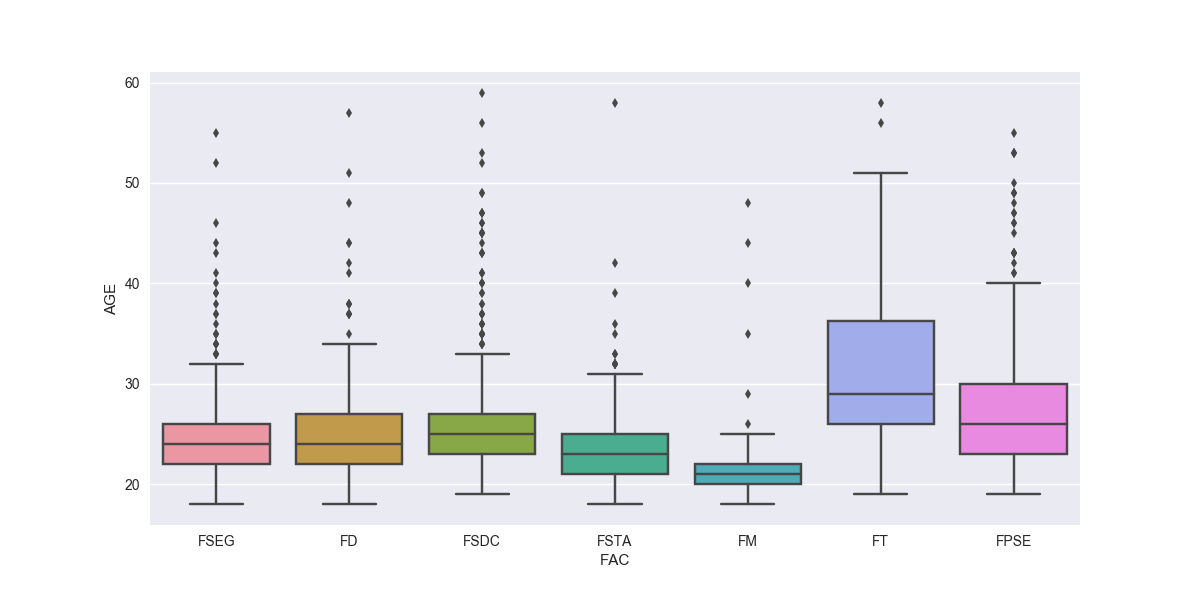
\includegraphics[width=0.8\textwidth]{fig/AGE-FAC.png}\label{fig:ANOVAb}
 	\caption{distribution des ages au sein des différentes facultés } 
 	\end{figure}
\subparagraph{Pourcentage}
  Également ici on rejette aussi notre hypothèse nulle qui stipulait que la
moyenne du pourcentage du diplôme est la même au sein de chaque faculté
. Pour prouver le rejet de notre hypothèse nulle , nous  pouvons remarquer que
les facultés de Médecine et celui de technologie ont une moyenne de
pourcentage de 59\% chacun et celui de théologie à une moyenne de 53\%.
\begin{table}[!htbp]
	\centering
	\begingroup % make the next setting local
	\captionsetup{type=table} % here we want to caption a table
	\caption{Analyse ANOVA pourcentage - faculté}
	\label{tab:ANOVAPourcentage}
	\begin{tabular}{lllllr}
		\toprule
		{} & df     &   sum\_sq &     mean\_sq      &     F    &     PR(>F) \\
		\midrule
		C(FAC)    &   6.0  &  9139.202728  &1523.200455  &48.757704&  2.256165e-58 \\
		Residual & 4708.0 & 147078.865397 &   31.240201  &      NaN      &     NaN \\
		\bottomrule
	\end{tabular}
	\endgroup
\end{table}
Pour Plus des détails sur les distributions statistique 
\begin{figure}[!htbp]
	\centering
	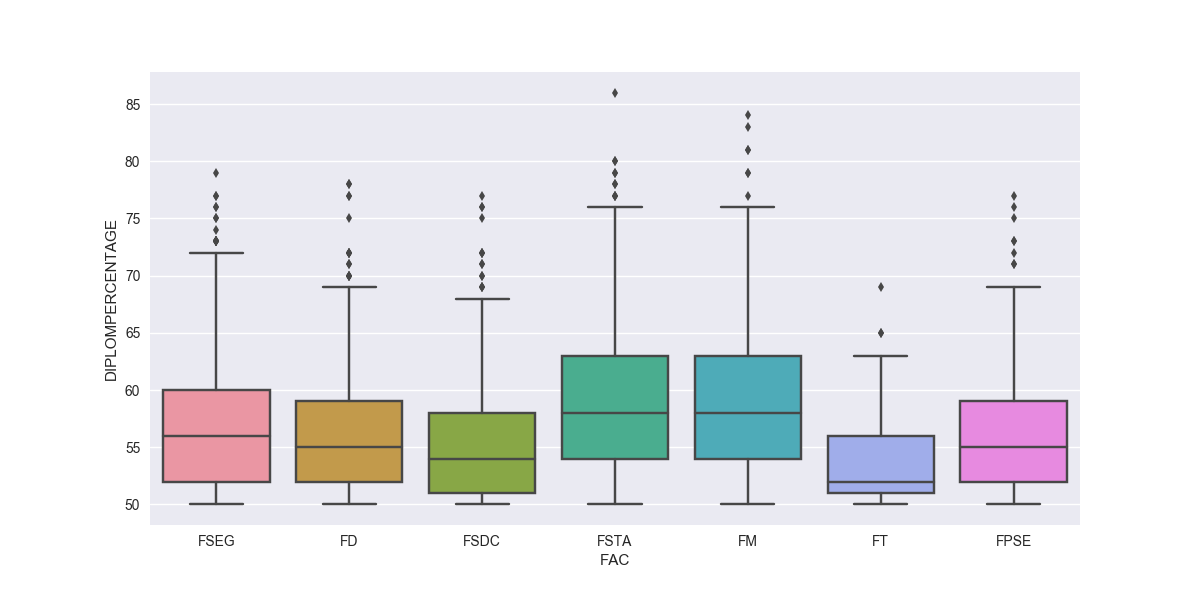
\includegraphics[width=0.8\textwidth]{fig/AGE-POURC.png}\label{fig:ANOVAa}
	\caption{distribution des pourcentage au sein des différentes facultés } 
\end{figure}
 \paragraph{Variables Catégorielles et Catégorielles}
 Pour ces genres de relations nous avons effectué le test chi-carré , Dans le tableau \ref{tab:chi-Carrée} nous pouvons visualiser les  différentes valeurs et effectuer nos conclusions sur base de celle ci.\\
 Notre hypothèse nulle H0 est du type : Il n'ya pas de relation entre la variable considérée et la faculté. 
 \begin{table}
 	\centering
 	\begingroup % make the next setting local
 	\captionsetup{type=table} % here we want to caption a table
 	\caption{Test chi carré entre  nos  différentes variables et la faculté }
 	\label{tab:chi-Carrée}
 	\begin{tabular}{lllllr}
 		\toprule
 		 Variable &   Dégrée De Lib.  &         Valeur Critique T & Valeur de Chi2 &  Décision sur H0 \\
 		\midrule
        Province & 90&113&256&Rejet\\
        Option & 174 & 205& 4155& Rejet \\
        SchoolStatus &42&58&304&Rejet\\
        SCHOOL&3558&3697&6389&Rejet\\
        SEXE&6&12,5&445&Rejet\\
 		\bottomrule
 	\end{tabular}
 	\endgroup
 \end{table}
 Voici les conclusions que nous prenons sur base de notre test statistique:
 \begin{enumerate}
 	\item FAC-PROVINCE :
 	lorsque nous comparons ces 2 valeurs , nous remarquons que notre valeur de chi2 est supérieure à notre valeur critique et tombe dans la région de rejet de notre hypothèse nulle et ainsi celle-ci est rejetée et ainsi nous concluons avec 95\% de certitude que notre hypothèse alternative est vrai: il ya une relation entre la province et la faculté en d'autre terme ayant un nombre des étudiant venant d'une province nous pouvons prédire la faculté choisie.
 	\item FAC-SEXE :
 il existe  une relation de dépendance entre le sexe et la faculté , ce qui est logique car par exemple en faculté de technologie et théologie on trouve moins des hommes que des femmes.
 	\item FAC-OPTION :
 	sur base de ce fait on fait la même conclusion que pour la province : il ya une relation de dépendance entre la section du diplôme et la faculté ce qui est logique car les étudiant en général se base sur leur option pour choisir leur faculté
 	\item FAC-SCHOOLSTATUS :
 	il existe  une relation de dépendance entre la section du diplôme et la faculté ce qui est logique car les étudiants en général se basent sur leur option pour choisir leur faculté
 \end{enumerate}
\paragraph{Analyse des données en entrée Vs le CGPA}:\\
Analysons enfin les relations existants entre nos données en entré et notre variable principale de sortie le \ac{CGPA}: 
comme à la partie précédente nous allons faire l'analyse Bi-variée  à
8 niveau mais au sein de chaque faculté et à la fin nous essayerons de voir l'analyse bi-varié entre nos 4 données de sortie 
\begin{enumerate}
	\item CGPA-Diplôme Province : Pour voir la relation entre le CGPA
	et la province d'origine de l'étudiant
	\item CGPA-DIPPOURCENTAGE: Pour voir
	la relation entre le CGPA et la pourcentage obtenu à \ac{EXETAT}
	\item CGPA-AGE: Pour voir la relation entre l'age de l'étudiant et le CGPA
	\item CGPA-FAC-DIPLOMEOPTION: Pour voir la relation entre le CGPA et l'option
	du diplôme mais par rapport aux faculté choisie.
	\item CGPA-FAC-SEXE: Pour
	la relation avec le sexe des étudiants et le CGPA Obtenu.
	\item  CGPA-FAC-SCHOOL: pour la relation entre l'école de provenance la fac 
	\item GPA-FAC-SCOOLSTATUS : pour la relation entre le statut de l'école de la
	FAC 
	\item FAC-CGPA
\end{enumerate}

Nos représenterons  les résultats su des divers tableaux dans les pages qui suivent.
\begin{table}
	\begingroup % make the next setting local
	\captionsetup{type=table} % here we want to caption a table
	\caption{Analyse entre les données d'entre et la donnée de sortie le CGPA en Faculté de Médecine}
	\label{tab:ANOVAMed}
	\noindent
	{\resizebox*{\textwidth}{\textheight}{%
			\renewcommand{\arraystretch}{2}
			\begin{tabularx}{\textwidth}{RRHJW}
				\toprule\rowcolor{white}
				\textbf{Variable}   & \textbf{Type}  & \textbf{P-value} & \textbf{Conclusion} &  \textbf{Commentaire}\\
				\hline
				\midrule
				PERC   & Pearson-Corr & 0.45 P=2 10e-5 & Pas de relation avec Le CGPA &  le coefficient étant inférieur à  0.5 conclu qu'il n'ya pas de corrélation considérable\\ 
				AGE   & Pearson-Corr & -0.26 P=6 10e-5 & Pas de relation avec Le CGPA &  le coefficient étant inférieur à  0.5 conclu qu'il n'ya pas de corrélation considérable , et comme le coefficient est négatif la corrélation es inverse\\
				STATUS   & ANOVA 1-way & 2 10 e-5 &< à 0.05  rejet de Ho les moyenne ne sont pas les même au sein de chaque catégorie &  Nous pouvons aisément remarqué que les étudiants venant des écoles catholiques réussissent mieux en faculté de médecine avec une moyenne de 60 ensuite viennent ceux des écoles protestantes\\
				SEXE   & ANOVA 1-way & 0.2 & >0.05 la moyenne du CGPA est la même Pour les hommes que pour les femmes  & le sexe n'as pas une influence considérable sur le CGPA bien que les filles ont des résultats légèrement meilleur  que les garçons en Faculté de médecine surtout en terme des distinctions \\
				SCHOOL & ANOVA 1-way & 0.009 & <0.05 rejet de Ho les moyenne ne sont pas les même au sein de chaque catégorie  & Après analyse des box-plot  des  20 écoles dont 10 sont les plus représentes et 5 sont ceux qui on une grande moyenne et 5 ceux qui ont une faible moyenne on remarque que les étudiant provenant des écoles comme lycée sainte Ursule, mwanga, Bakanja ,ALfagiri, faraja,amani, n'échouent presque pas en faculté de médecine\\
				OPTION &ANOVA 1-way &0.4 & >0.05 	on n'accepte pas l'hypothèse nulle immédiatement ,&  la moyenne est la même que pour certaines options  Bio-chimie, nutrition , agricole on la même ,mais certains Option on une moyenne plus élevé que d'autres Notre CGPA dépend aussi de l'option du diplôme \\
				\bottomrule
	\end{tabularx}}}
\endgroup
\end{table}
\begin{table}
	\centering
	\begingroup % make the next setting local
	\captionsetup{type=table} % here we want to caption a table
	\caption{Analyse entre les données d'entre et la donnée de sortie le CGPA en Faculté de Technologie}
	\label{tab:ANOVATech}
	\noindent
	{\resizebox*{\textwidth}{\textheight}{%
			\renewcommand{\arraystretch}{2}
			\begin{tabularx}{\textwidth}{RRHJW}
				\toprule\rowcolor{white}
				\textbf{Variable}   & \textbf{Type}  & \textbf{P-value} & \textbf{Conclusion} &  \textbf{Commentaire}\\
				\hline
				\midrule
				PERC   & Pearson-Corr & 0.34P=2 10e-5 & Pas de relation avec Le CGPA &  le coefficient étant inférieur à  0.5 conclu qu'il n'ya pas de corrélation considérable\\ 
				
				AGE   & Pearson-Corr & -0.03 P=6 10e-5 & Pas de relation avec Le CGPA &  le coefficient étant inférieur à  0.5 conclu qu'il n'ya pas de corrélation considérable , et comme le coefficient est négatif la corrélation es inverse\\
				
				SEXE   & ANOVA 1-way & 0.081204 & >0.05 la moyenne du CGPA est la même Pour les hommes que pour les femmes  . Mais la faculté est plus maculine avec 85\% des Hommes et 15\% des Femmes de& le sexe n'as pas une influence considérable sur le CGPA en faculté de technologie appliquée , les deux catégories ont presque la même moyenne \\
				
				PROVINCE   & ANOVA 1-way &0.07731&> à 0.05  On n'accepte pas H0 Automatiquement , Certaines catégories on la même Moyenne &  après analyse graphique on conclu Rapidement que les étudiants provenant de la province du sud Kivu sont plus performant en faculté de Technologie\\
				
				STATUS   & ANOVA 1-way & 3.12e-13&< à 0.05  rejet de Ho les moyenne ne sont pas les même au sein de chaque catégorie & Nous remarquons que les étudiant venant des écoles catholiques  réussissent mieux en faculté de Techno , ensuite les autodidacte ,ensuite ceux des écoles protestantes\\
				
				SCHOOL & ANOVA 1-way & 3.939e-11& <0.05 rejet de Ho les moyenne ne sont pas les même au sein de chaque catégorie  & On remarques sur la figure que les grandes écoles connus on une bonne moyenne et un bon maximum de CGPA comme le lycée Amani, l'ITIG , l'ITFM,etc..\\
				
				OPTION &ANOVA 1-way &1.05e-23&  <0.05 rejet de Ho les moyenne ne sont pas les même au sein de chaque catégorie  ,& Comme nous pourrions s'y attendre les options techniques et Scientifiques viennent en tête de liste et en bas de l'échelle viennent  les options littéraires et commerciales \\
				
				\bottomrule
	\end{tabularx}}}
	\endgroup
\end{table}
\begin{table}
	\centering
	\begingroup % make the next setting local
	\captionsetup{type=table} % here we want to caption a table
	\caption{Analyse entre les données d'entre et la donnée de sortie le CGPA en Faculté de d'économie}
	\label{tab:ANOVAEco}
	{\resizebox*{\textwidth}{\textheight}{%
			\renewcommand{\arraystretch}{2}
			\begin{tabularx}{\textwidth}{RRHJW}
				\toprule\rowcolor{white}
				\textbf{Variable}   & \textbf{Type}  & \textbf{P-value} & \textbf{Conclusion} &  \textbf{Commentaire}\\
				\hline
				\midrule
				PERC   & Pearson-Corr & 0.236P=2 10e-5 & Pas de relation avec Le CGPA &  le coefficient étant inférieur à  0.5 conclu qu'il n'ya pas de corrélation considérable\\ 
				 
				AGE   & Pearson-Corr & -0.08 P=6 10e-5 & Pas de relation avec Le CGPA &  le coefficient étant inférieur à  0.5 conclu qu'il n'ya pas de corrélation considérable , et comme le coefficient est négatif la corrélation es inverse\\
				 
				SEXE   & ANOVA 1-way & 0.585536 & >0.05 la moyenne du CGPA est la même Pour les hommes que pour les femmes. La faculté a 54\% des Hommes et 46\% des Femmes & le sexe n'as pas une influence considérable sur le CGPA . Les deux catégorie ont une même moyenne\\
				 
				PROVINCE   & ANOVA 1-way &0.07731&> à 0.05  On n'accepte pas H0 Automatiquement , Certaines catégories on la même Moyenne &  après analyse graphique on conclu Rapidement que les étudiants provenant de la province du Nord Kivu sont plus performant en faculté d'économie , ensuite vient la province du Sud-Kivu, en bas de l'échelle nous trouvons la province du Kasai\\
				 
				STATUS   & ANOVA 1-way & 2.21e-13&< à 0.05  rejet de Ho les moyenne ne sont pas les même au sein de chaque catégorie & Nous remarquons que les étudiant venant des écoles catholiques  réussissent mieux en faculté d'économie, ensuite les autodidacte ,ensuite ceux des écoles protestantes\\
				 
				SCHOOL & ANOVA 1-way & 2.939e-11& <0.05 rejet de Ho les moyenne ne sont pas les même au sein de chaque catégorie  & On remarques sur la figure que les grandes écoles connus on une bonne moyenne et un bon maximum de CGPA comme le lycée Amani, l'ITIG , l'ITFM, etc..\\
				 
				OPTION &ANOVA 1-way &3.53e-12&  <0.05 rejet de Ho les moyenne ne sont pas les même au sein de chaque catégorie  ,& Contrairement aux idées réussies ne les options techniques et Scientifiques viennent en tête de liste ensuite vienne les options économies , commerciale et latin philo .En bas de l'échelle vienne les options sociales et pédagogiques \\
				 
				\bottomrule
	\end{tabularx}}}
	\endgroup
\end{table}
\begin{table}
	\centering
	\begingroup % make the next setting local
	\captionsetup{type=table} % here we want to caption a table
	\caption{Analyse entre les données d'entre et la donnée de sortie le CGPA en Faculté de Droit}
	\label{tab:ANOVADroit}
	{\resizebox*{\textwidth}{\textheight}{%
			\renewcommand{\arraystretch}{2}
			\begin{tabularx}{\textwidth}{RRHJW}
				\toprule\rowcolor{white}
				\textbf{Variable}   & \textbf{Type}  & \textbf{P-value} & \textbf{Conclusion} &  \textbf{Commentaire}\\
				 \hline
				 \midrule
				PERC   & Pearson-Corr & 0.22P=2 10e-5 & Pas de relation avec Le CGPA &  le coefficient étant inférieur à  0.5 conclu qu'il n'ya pas de corrélation considérable\\ 
				 
				AGE   & Pearson-Corr & 0.11 4 P=6 10e-5 & Pas de relation avec Le CGPA &  le coefficient étant inférieur à  0.5 conclu qu'il n'ya pas de corrélation considérable , et comme le coefficient est négatif la corrélation es inverse\\
				 
				SEXE   & ANOVA 1-way &0.745 & >0.05 la moyenne du CGPA est la même Pour les hommes que pour les femmes. La faculté a 60\% des Hommes et 40\% des Femmes & le sexe n'as pas une influence considérable sur le CGPA . Les deux catégorie ont une même moyenne\\
				 
				PROVINCE   & ANOVA 1-way &0.187473&>0.05 On accepte pas automatiquement H0 on observe de plus prêt & Nous remarquons que le moyenne du CGPA est la même pour les provinces suivantes : Nord-Kivu, Sud-Kivu, Kinshasa , Orientale ,Maniema, les distinctions proviennent beaucoup plus des provinces du nord-Kivu, sud Kivu et Kinshasa.\\
				 
				STATUS   & ANOVA 1-way &	1.20e-08& >0.05 la moyenne pour les différentes statut n'est pas la même  &  Nous remarquons que les celles étudiants qui distinguent c'est ceux provenant des écoles protestants et catholiques, en queue de la liste se trouve les autodidacte\\
				 
				SCHOOL & ANOVA 1-way &2.5e-10& < 0.05 la moyenne n'est pas la même  & CGPA dépend de cette valeur car certains écoles échouent lamentablement d'autres pas\\
				 
				OPTION &ANOVA 1-way &7.25e-10&  < 0.05 la moyenne n'est pas la même  & Voila comme on pourrait s'y attendre l'option latin philo est en tête de liste les options commerciale , pédagogie , sociale , math-physique ,mec sont en bas de l'échelle \\
				 
				\bottomrule
	\end{tabularx}}}
	\endgroup
\end{table}

\begin{table}
	\centering
	\begingroup % make the next setting local
	\captionsetup{type=table} % here we want to caption a table
	\caption{Analyse entre les données d'entre et la donnée de sortie le CGPA en Faculté de Santé}
	\label{tab:ANOVASante}
	{\resizebox*{\textwidth}{\textheight}{%
			\renewcommand{\arraystretch}{2}
			\begin{tabularx}{\textwidth}{RRHJW}
				\toprule\rowcolor{white}
				\textbf{Variable}   & \textbf{Type}  & \textbf{P-value} & \textbf{Conclusion} &  \textbf{Commentaire}\\
				\hline
				\midrule
				PERC   & Pearson-Corr & 0.236 P=2 10e-5 & Pas de relation avec Le CGPA &  le coefficient étant inférieur à  0.5 conclu qu'il n'ya pas de corrélation considérable\\ 
				 
				AGE   & Pearson-Corr & -0.06 P=6 10e-5 & Pas de relation avec Le CGPA &  le coefficient étant inférieur à  0.5 conclu qu'il n'ya pas de corrélation considérable , et comme le coefficient est négatif la corrélation es inverse\\
				 
				SEXE   & ANOVA 1-way & 0.17 & >0.05 la moyenne du CGPA est la même Pour les hommes que pour les femmes. La faculté a 40\% des Hommes et 60\% des Femmes & le sexe n'as pas une influence considérable sur le CGPA . Les deux catégorie ont une même moyenne\\
				 
				PROVINCE   & ANOVA 1-way &0.089&> à 0.05  On n'accepte pas H0 Automatiquement , Certaines catégories on la même Moyenne &  La tendance est inversée les étudiant de la province du sud et nord kivu échouent plus en faculté de santé, les distinctions proviennent de la province orientale et du sud Kivu.\\
				 
				STATUS   & ANOVA 1-way & 8 10e-5&< à 0.05  rejet de Ho les moyenne ne sont pas les même au sein de chaque catégorie & Nous remarquons que les étudiant venant des écoles catholiques , protestantes en tête de liste , mais les écoles musulmanes , privé , et autodidacte viennent en bas de l'échelle\\
				 
				SCHOOL & ANOVA 1-way & 0.00223& <0.05 rejet de Ho les moyenne ne sont pas les même au sein de chaque catégorie  & Les étudiant provenant des écoles suivantes échouent rarement faculté de santé : Maendeleo, sainte ursule , Bakandja.\\
				 
				OPTION &ANOVA 1-way &1e-6&  <0.05 rejet de Ho les moyenne ne sont pas les même au sein de chaque catégorie  ,& Les Options scientifiques , techniques réussissent mieux au sein de la faculté de santé \\
				 
				\bottomrule
		\end{tabularx}}}
		\endgroup
	\end{table}
	
	\begin{table}
		\centering
		\begingroup % make the next setting local
		\captionsetup{type=table} % here we want to caption a table
		\caption{Analyse entre les données d'entre et la donnée de sortie le CGPA en Faculté de Psychologie}
		\label{tab:ANOVAPscyco}
		{\resizebox*{\textwidth}{\textheight}{%
				\renewcommand{\arraystretch}{2}
				\begin{tabularx}{\textwidth}{RRHJW}
					\toprule\rowcolor{white}
					\textbf{Variable}   & \textbf{Type}  & \textbf{P-value} & \textbf{Conclusion} &  \textbf{Commentaire}\\
					 \hline
					 \midrule
					PERC   & Pearson-Corr & 0.32 P=2 10e-5 & Pas de relation avec Le CGPA &  le coefficient étant inférieur à  0.5 conclu qu'il n'ya pas de corrélation considérable\\ 
					 
					AGE   & Pearson-Corr & 0.09 P=6 10e-5 & Pas de relation avec Le CGPA &  le coefficient étant inférieur à  0.5 conclu qu'il n'ya pas de corrélation considérable , et comme le coefficient est négatif la corrélation es inverse\\
					 
					SEXE   & ANOVA 1-way &0.603 & >0.05 la moyenne du CGPA est la même Pour les hommes que pour les femmes. La faculté a 48\% des Hommes et 52\% des Femmes & le sexe n'as pas une influence considérable sur le CGPA . Les deux catégorie ont une même moyenne\\
					 
					PROVINCE   & ANOVA 1-way &0.585&> à 0.05  On n'accepte pas H0 Automatiquement , Certaines catégories on la même Moyenne &  Nous remarquons que le moyenne du CGPA est la même pour les provinces suivantes : Nord-Kivu, Sud-Kivu, Kinshasa , Orientale ,Maniema, les distinctions proviennent beaucoup plus des provinces du nord-Kivu, sud-Kivu .\\
					 
					STATUS   & ANOVA 1-way & 0.017&< à 0.05  rejet de Ho les moyenne ne sont pas les même au sein de chaque catégorie & les étudiants issue des écoles privées catholiques, et protestantes obtiennent des bonnes notes au sein de la faculté de Pycho, on remarque que ceux issues des écoles catholiques échouent moins\\
					 
					SCHOOL & ANOVA 1-way & 0.000061& <0.05 rejet de Ho les moyenne ne sont pas les même au sein de chaque catégorie  & Les étudiant provenant des écoles suivantes échouent rarement faculté de psychologie : Maendeleo, sainte ursule , Bakandja ,amani , meta Anuarite.\\
					 
					OPTION &ANOVA 1-way &0.000214&  <0.05 rejet de Ho les moyenne ne sont pas les même au sein de chaque catégorie  ,& contrairement aux idées réussies ceux qui réussissent plus en faculté de psychologie sont les étudiant issues des section scientifiques ensuite vient 'option latin philo et en 4ème position l'option pédagogique , signalons su'aucun étudiant issu de commerciale n'as réussi au sein de cette faculté \\
					 
					\bottomrule
		\end{tabularx}}}
		\endgroup
	\end{table}
	
	\begin{table}
		\centering
		\begingroup % make the next setting local
		\captionsetup{type=table} % here we want to caption a table
		\caption{Analyse entre les données d'entre et la donnée de sortie le CGPA en Faculté de Théologie}
		\label{tab:ANOVATheo}
		{\resizebox*{\textwidth}{\textheight}{%
				\renewcommand{\arraystretch}{2}
				\begin{tabularx}{\textwidth}{RRHJW}
					\toprule\rowcolor{white}
					\textbf{Variable}   & \textbf{Type}  & \textbf{P-value} & \textbf{Conclusion} &  \textbf{Commentaire}\\
					 \hline
					 \midrule
					PERC   & Pearson-Corr & 0.14P=2 10e-5 & Pas de relation avec Le CGPA &  le coefficient étant inférieur à  0.5 conclu qu'il n'ya pas de corrélation considérable\\ 
					 
					AGE   & Pearson-Corr & 0.14 P=6 10e-5 & Pas de relation avec Le CGPA &  le coefficient étant inférieur à  0.5 conclu qu'il n'ya pas de corrélation considérable , et comme le coefficient est négatif la corrélation es inverse\\
					 
					SEXE   & ANOVA 1-way &0.745 & >0.05 la moyenne du CGPA est la même Pour les hommes que pour les femmes. La faculté a 80\% des Hommes et 20\% des Femmes & le sexe n'as pas une influence considérable sur le CGPA . Les deux catégorie ont une même moyenne\\
					 
					PROVINCE   & ANOVA 1-way &0.033&< à 0.05  nous pouvons conclure que la moyenne n'est pas la même au sein de chaque faculté &  Les résultats remarquables viennent des provinces du sud-Kivu, du nord-Kivu et de la province orientale\\
					 
					STATUS   & ANOVA 1-way &0.717429& >0.05 On accepte pas automatiquement H0 on observe de plus prêt   &  Contrairement aux idées réussies les étudiant On serait tenter de dire que les étudiants issues des écoles protestantes réussissent mieux au sein de cette faculté mais les statistiques nous prouvent le contraire\\
					 
					SCHOOL & ANOVA 1-way &0.156736& >0.05 On accepte pas automatiquement H0 on observe  & CGPA dépend de cette valeurs car certains écoles échouent lamentablement d'autres pas\\
					 
					OPTION &ANOVA 1-way &0.356&  .05 On accepte pas automatiquement H0 on observe& Les échecs sont des cas rare au sein de cette faculté , et que tous le monde réussi mieux \\
					 
					\bottomrule
		\end{tabularx}}}
		\endgroup
	\end{table}
\newpage 
\section{Conclusion partielle}
Nous avons à présent notre ensemble d'apprentissage avec nos variables en entrée et les variables en sortie bien nettoyées, nous avons d'analysé 
les corrélations existantes entre les variables d'entrées et le choix de la faculté , ensuite celles existantes avec le CGPA notre variable principale !
\paragraph{}
Dans la première phase de l'analyse bi-varié nous avons pu conclure que tous nos variables avaient une influence  sur le choix de la Faculté;
par exemple les femmes ne choisissent pas les facultés de Technologie et Théologie plus fréquemment, les étudiants issus des sections scientifiques et techniques s'orientent plus en faculté de technologie ,les étudiants les plus agés sont en faculté de théologie, le moins agés sont en faculté de médecine, ceux avec un grand pourcentage à l'\ac{EXETAT} sont en faculté de Médecine et technologie.
\paragraph{}
Mais après l'analyse de ces données face à notre variable de sortie le CGPA celle qui symbolise le réussite d'un étudiant au sein d'une faculté nous avons pu remarque avec certitude que certaines variables n'influent à rien sur le CGPA comme le pourcentage obtenu à l'\ac{EXETAT}  ,l'age ainsi que le sexe des étudiant!
C'est pourquoi lors de l'élaboration de  notre modèle d'apprentissage ses variables ne seront pas considérés lors de la constitution de notre ensemble d'apprentissage surtout pour la prédiction du CGPA. \\
Nous passons maintenant au prochain chapitre consistant à l'élaboration de notre ensemble d'apprentissage et notre modèle de prédiction  pour chaque faculté.